
\documentclass{article}
\usepackage{amsmath}
\usepackage[margin=2cm]{geometry}
\usepackage[T1]{fontenc}
\usepackage{listings}
\usepackage{graphicx}

\setlength{\parskip}{10pt plus 2pt minus 2pt}

\title{3D Random Walk}
\author{LYU Liuke}
\date{PHYS3061: Lab Report 1}

\begin{document}

\maketitle
\tableofcontents
\clearpage

\section{Introduction}

\subsection{Random Number Generator}

The random number generator implemented here is a simple Linear Congruential
Generator(LCG), which is generally a recursive mapping within a certain integer
domain. for a set of parameters (a,c,m):

\begin{align*}
  x_{N+1} &= (x_N * a + c) \mod m \\
  \xi \colon \{1,2,3,\dots,m-1\} &\to \{1,2,3,\dots,m-1\}
\end{align*}

Some special sets of (a,c,m) give seemingly very random and uniform distribution
of results in recursive mapping. Based on this feature, we consider this recursive 
method as a random number generator. 

In this experiment (a=1559, c=647, m=13229) are chosen. 
The main characteristic of these parameters is that they are all primes, in order
to try to avoid periodicity behaviors in the random sequance.
This special set is chosen by testing different combinations of (a,c,m) in a
small parameter space.

\subsection{Random Walk}
  
A random walk, in simple terms, is a random sequance representing the 
accumulative sum of a random variable. In a simple 3D case:

\begin{align*}
  \vec{X_N} &= \sum_{i=1}^{n} \vec{s_i} \\
  \mbox{where} \quad  \vec{s} \in V &= \{(1,0,0), (-1,0,0), (0,1,0), (0,-1,0), (0,0,1),(0,0,-1)\} \\
  \mbox{Assigning} \quad P(\vec{v}) &\equiv 1/6 \quad \mbox{for}  \quad \vec{v} \in V
\end{align*}

Probability analysis give this famous relationship:

\begin{align*}
  <|\vec{X_N}|^2> = \sqrt{N} 
\end{align*}

This relationship can be verified by a Monte Carlo Method, averaging the results
over a large number of samples. Alternatively, we can use it to evaluate the 
randomness of our LCG generator.
\section{Code}

\subsection{Linear Congruential Generator}

\lstinputlisting[language=Python,firstline=8, lastline=23]{lab1.py}

LCG is the linear congruential generator with parameters a=1559, c=313 (647),
m=13229. The seed of the generator is determined by decimal time. The structure of it
is a python generator, which is a sequance of predefined operations. This gives a good 
structure to continuously generate any length of random numbers and also avoids defining
a global state variable. The outputs of this function (after "yield") is normalized to 
(0,1) by dividing it by m. 

\subsection{3D Random Walk}

\lstinputlisting[language=Python,firstline=29, lastline=37]{lab1.py}

\lstinputlisting[language=Python,firstline=52, lastline=66]{lab1.py}

As can be seen, I created two versions of random walk function, one with uniform random
floating step size and the other with fixed integer step size. They are for different 
types of purposes, and requires different set of parameters of LCG to get reasonable 
results. Since function RandomWalk\_fs is by nature a mere assembling of three 
mutually independent 1D random walks, I tend to use the second one in which each step
the walker randomly choose a direction among x, y, z and randomly chooses to go 1 step
forward or backward. In such case, the three axes are no longer independent.

In the second function, I made use of another function random\_choice, which is a 
mimic of np.random.choice function, but with my LCG as the random number generator.

\section{Application}

\subsection{P\'olya's Random Walk Problem}

In this part we make use of the function RandomWalk to solve a problem named after  
P\'olya. The problem is:

\begin{center}
	\textit{
	For a random walk on a n-dimensional lattice, what is the probability of it
	returning to the origin?
	}
\end{center}

Since this is a lattice random walk, each step shall be a fixed integer step along one
of the three normal directions, we shall use function RandomWalk. The script I used for
this problem is called returning.py

The idea is simple, we conduct a large number of random walks (10000 particles) of 
sufficient steps (20000 steps), and record how many of them comes back. We conduct 
this experiment several times (10 times), and if the resultant probability have a small 
enough standard deviation, we believe that this result is close to the theoretical 
prediction. I conducted this experiment for dimension 1 - 5, the results are as follows:

\begin{center}
\begin{tabular}{ c c c c }
	dim & p\_exp(d) & std & p(d) \\
	1 & 0.9941& 0.0007& 1 \\
	2 & 0.753& 0.003& 1 \\
	3 & 0.337& 0.005& 0.340537 \\
	4 & 0.193& 0.005& 0.193206 \\
	5 & 0.134& 0.002& 0.135178
\end{tabular}
\end{center}

\section{Results and Analysis}

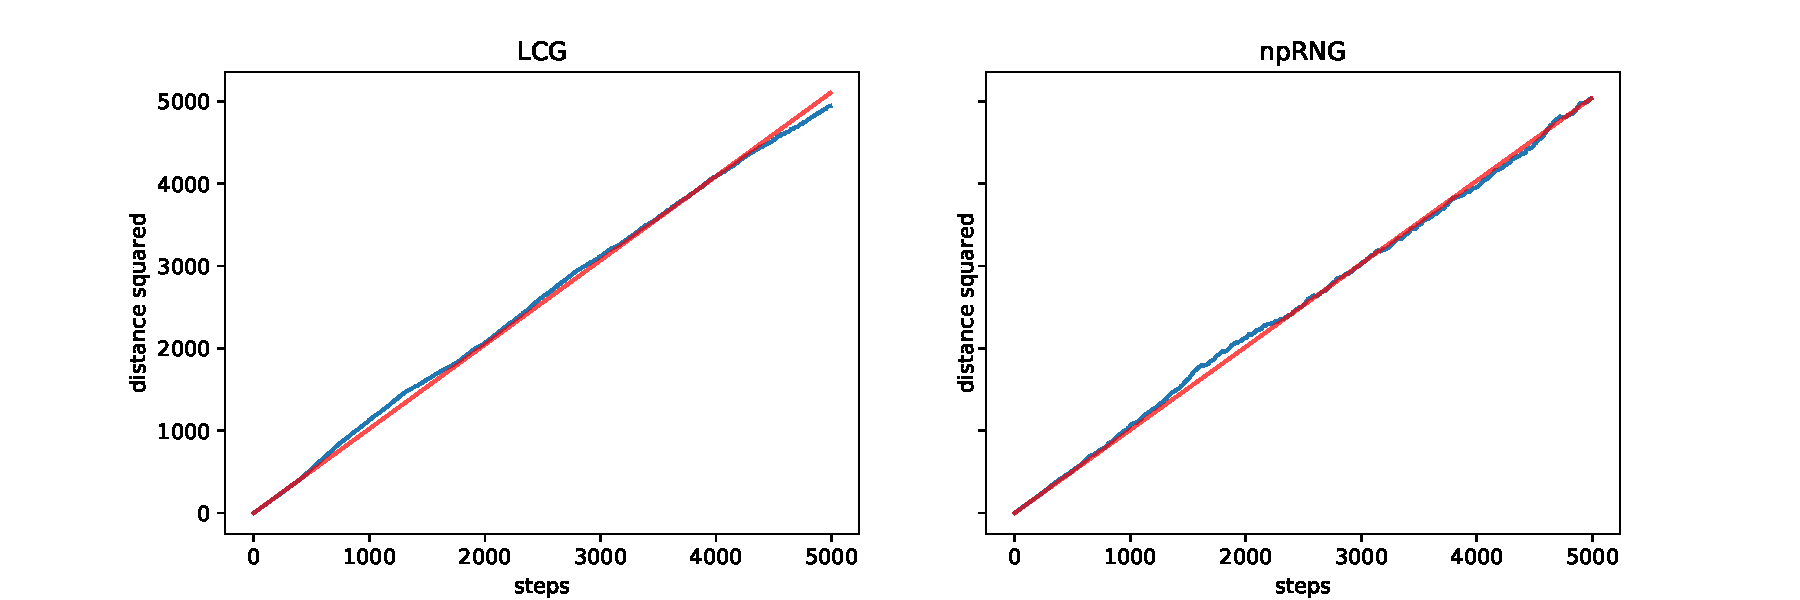
\includegraphics[width=\textwidth]{linear.pdf}

\section{Conclusion}

\begin{thebibliography}{1}
  \bibitem{table} Weisstein,Eric W. "P\'olya's Random Walk Constants." From MathWorldld: A Wolfram Web Resource. http://mathworld.wolfram.com/PolyasRandomWalkConstants.html
 }
\end{thebibliography}

\end{document}

\iffalse
  Your Report should include
- Brief introduction of random number generator and random walk (less than one page)
- Present the parameter you used and outline your codes
- Results and analysis. (Proper figures or tables should be included to show the results)
- Conclusion

\fi
